% ---------------------------------------------------------------------------
% Results panel.  Every number here comes from the implementation repository
% (tool 1.0.0): the benchmark rows of evaluation/results.csv and the
% RMC-generated fixtures under src/test/resources/rebeca-generated.  Nothing is
% retyped from prose.
%
% The callout reports the runs as an observation, not as a property of the
% algorithm.  The mean is the unweighted mean of the eleven per-run state
% reduction ratios (16.7, 30.0, 37.5, 50.0, 60.0, 66.7, 69.6, 71.4, 76.2,
% 89.5, 89.5 -> 59.7%), rounded, and it is stated together with what it does
% not establish: neither that a minimal quotient is unique under weak timed
% bisimulation, nor that what the tool builds is minimal.  That the tool
% re-checks its own output is not reported here -- it is the premise of the
% problem, not a finding.
% ---------------------------------------------------------------------------
\newcommand{\ResultsContent}{%

\vspace{-.30cm}
\PosterHighlight[PosterGreen]{%
\PosterLead{آنچه در نمونه‌ها دیده شد:} به‌طور میانگین حدود \pct{60} از حالت‌ها حذف
شده‌اند، و بیان‌های متفاوت یک رفتار --- با اندازه‌های بسیار متفاوت --- به مدل
خارج‌قسمتی یکسانی رسیده‌اند.

\vspace{.12cm}
این ثابت نمی‌کند که خارج‌قسمتِ کمینه تحت این رابطه یکتاست، یا اینکه آنچه ابزار
می‌سازد کمینه است؛ اما شاهدی است که دنبال‌کردن این اثبات را موجه می‌کند.}

{\postertitlefont\fontsize{28}{36}\selectfont
دو بیان هم‌ارز و خارج‌قسمت مشترکشان\par}
\vspace{.12cm}

تنها \code{mood.LAUGH} و \code{mood.CRY} قابل مشاهده‌اند. \code{mood1} انتظار را
به دو گام می‌شکند و میانشان یک پیام پنهان دارد؛ \code{mood2} همان دوره را یکپارچه
می‌گذراند.

\vspace{.22cm}
\begin{center}
\begin{minipage}[b]{7.3cm}
  \centering
  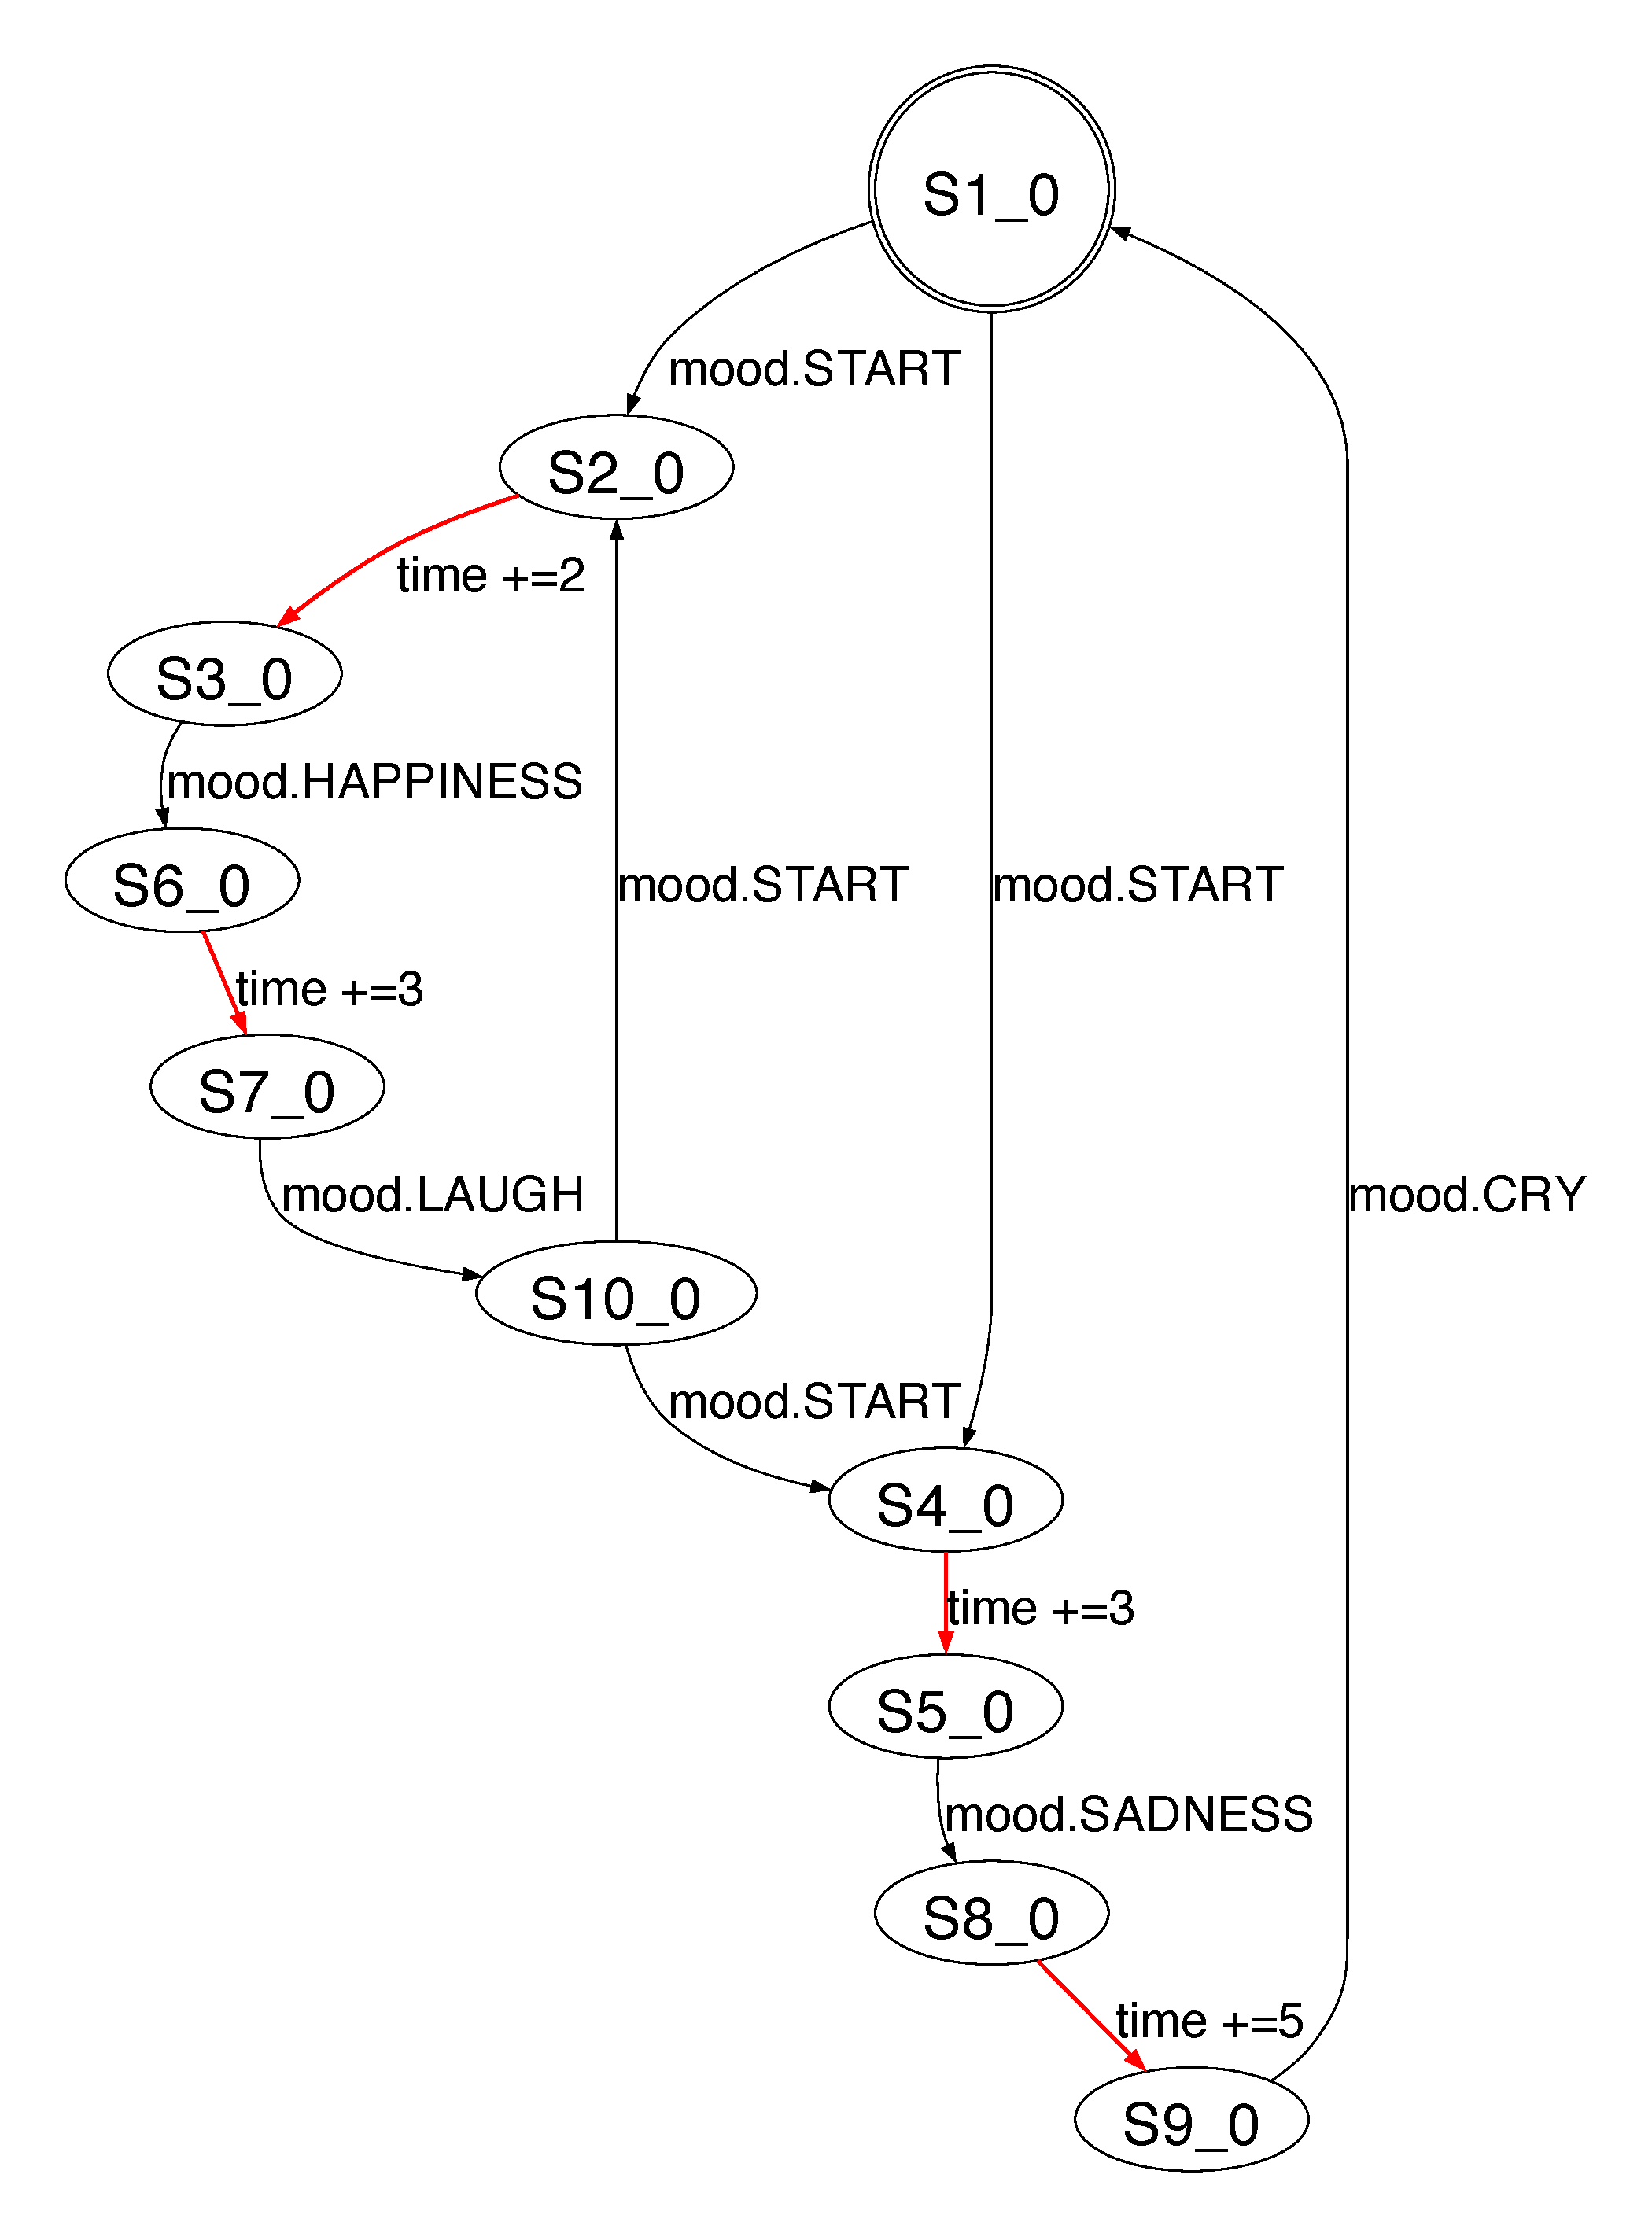
\includegraphics[width=7.3cm]{assets/figures/mood1.pdf}\par
  \vspace{.20cm}
  {\fontsize{22}{27}\selectfont\color{PosterPurple}\bfseries\code{mood1}\par}
  {\fontsize{19}{24}\selectfont ۱۰ حالت، ۱۲ گذار\par}
\end{minipage}%
\hfill
\begin{minipage}[b]{1.2cm}
  \centering
  {\fontsize{34}{40}\selectfont\color{PosterPurple}$\boldsymbol{\approx}$\par}
  \vspace{4.6cm}
\end{minipage}%
\hfill
\begin{minipage}[b]{10.7cm}
  \centering
  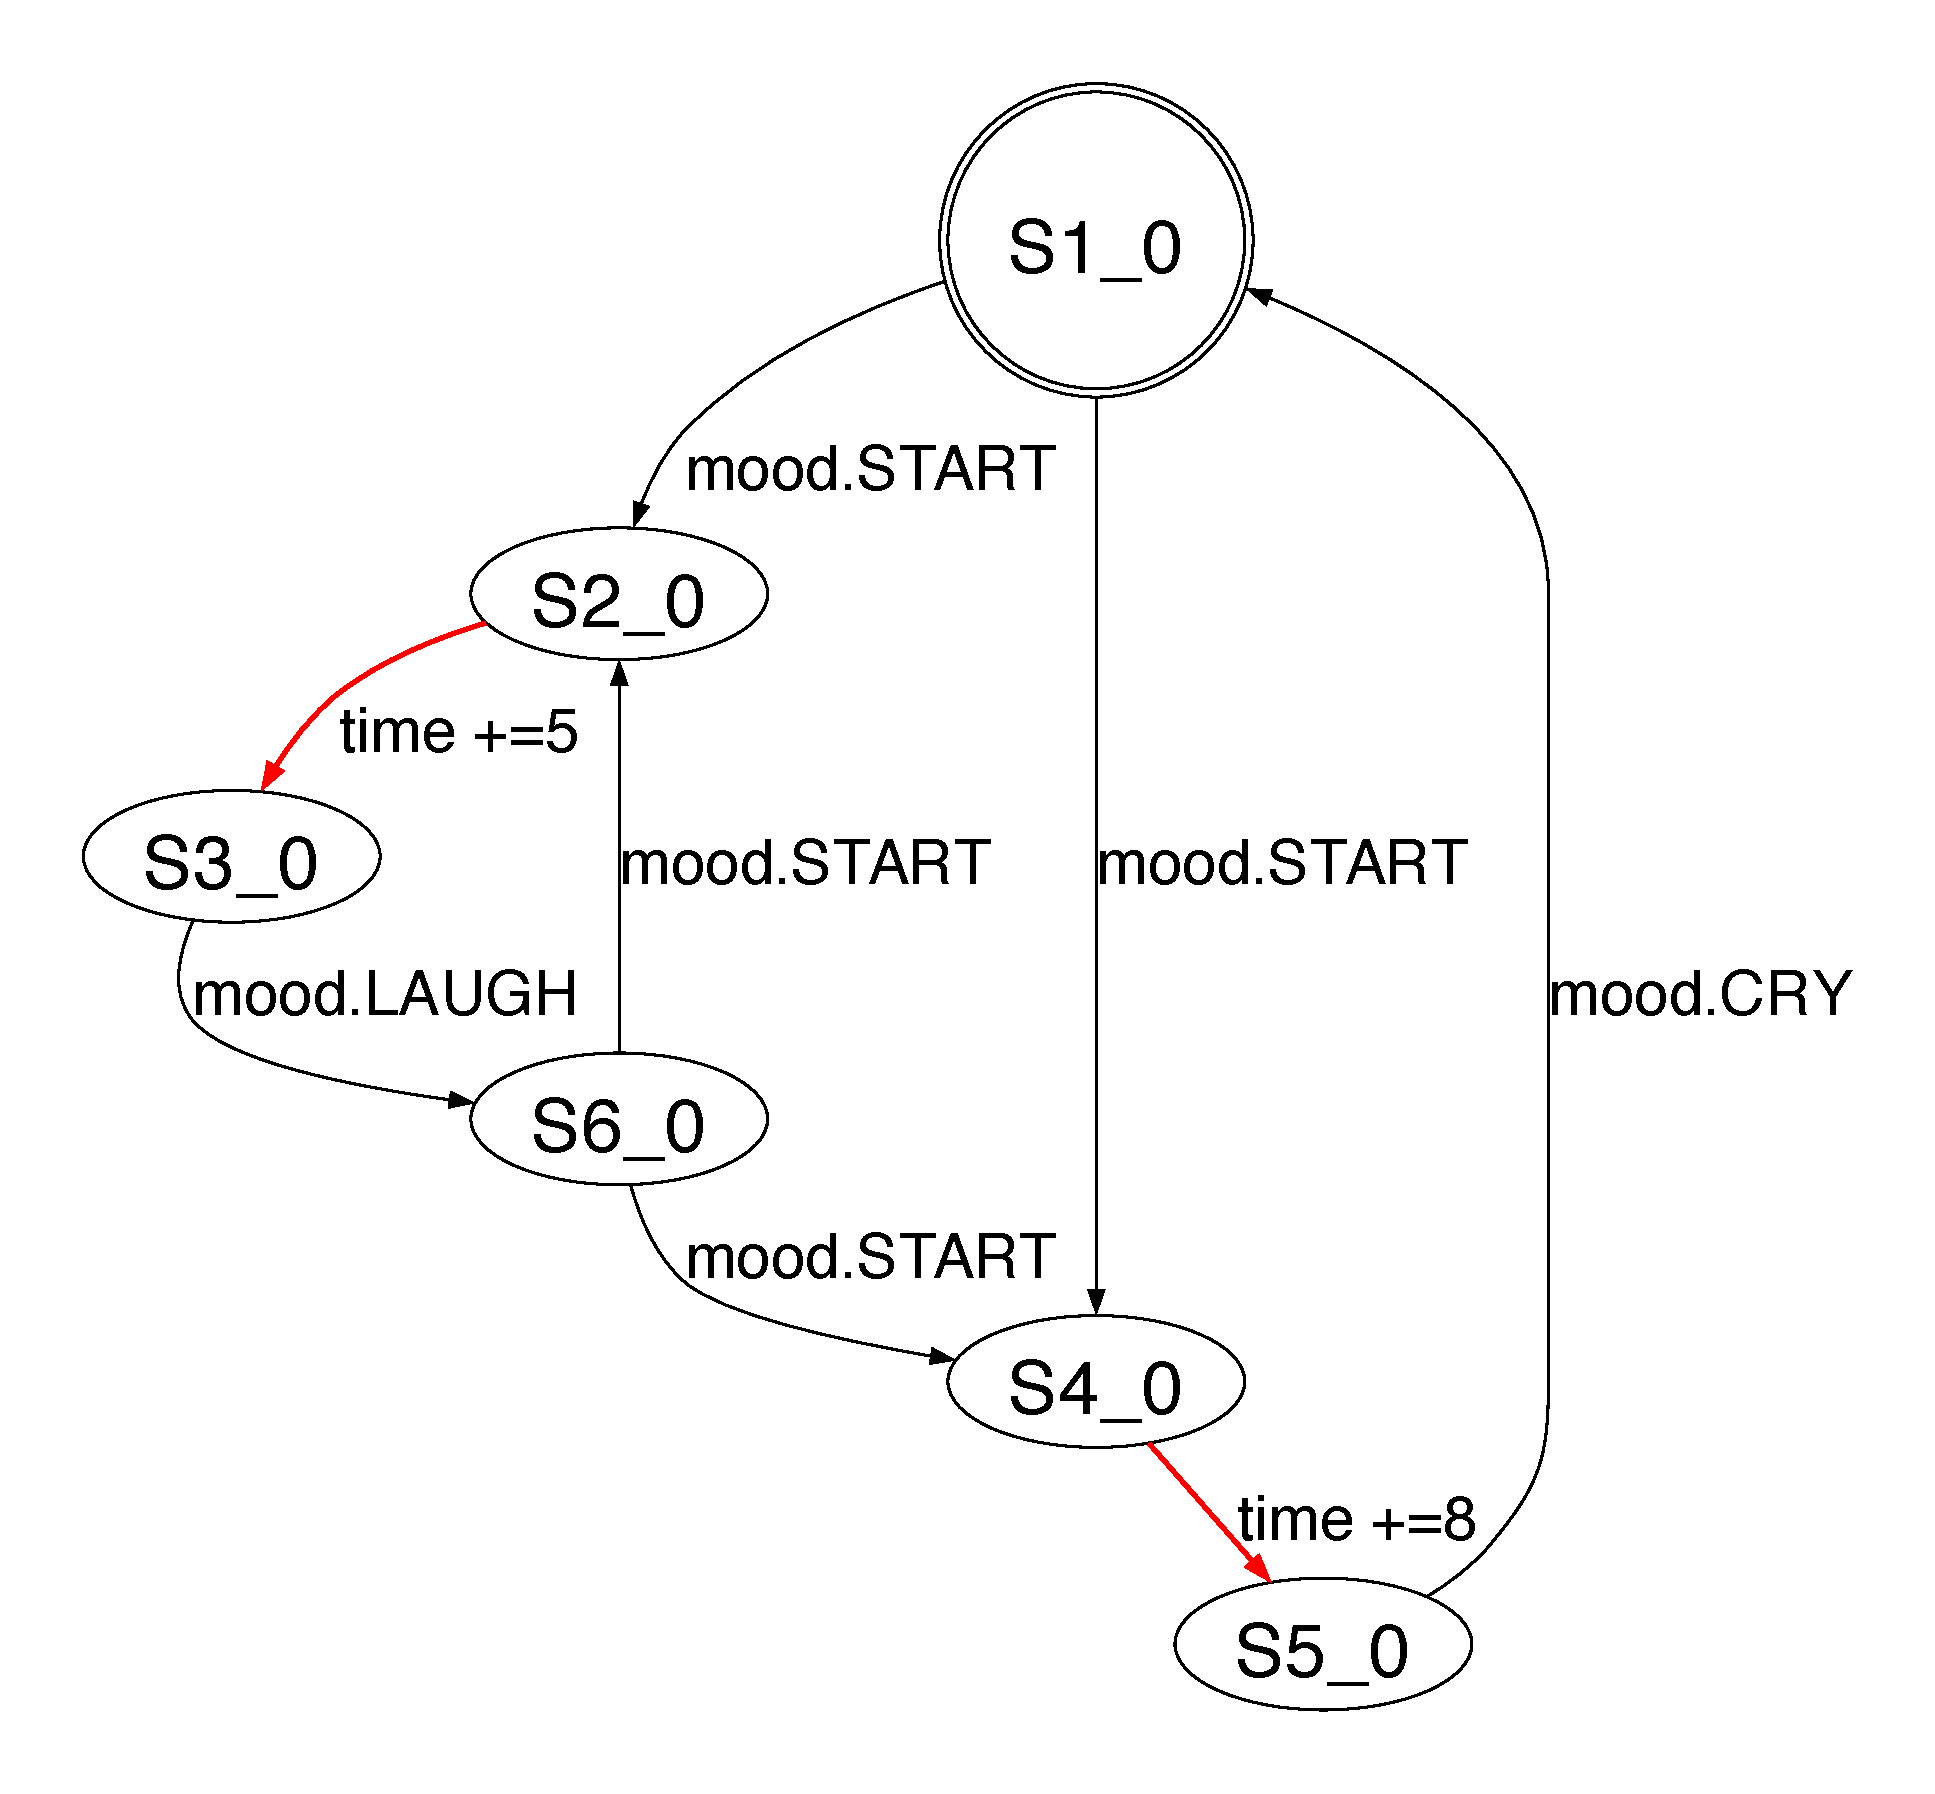
\includegraphics[width=10.7cm]{assets/figures/mood2.pdf}\par
  \vspace{.20cm}
  {\fontsize{22}{27}\selectfont\color{PosterPurple}\bfseries\code{mood2}\par}
  {\fontsize{19}{24}\selectfont ۶ حالت، ۸ گذار\par}
\end{minipage}
\end{center}

\vspace{.22cm}
{\centering
{\fontsize{21}{27}\selectfont\color{PosterGreen}\bfseries
 $\boldsymbol{\downarrow}$\; هر دو به همین یک مدل کاهش می‌یابند\par}
\vspace{.18cm}
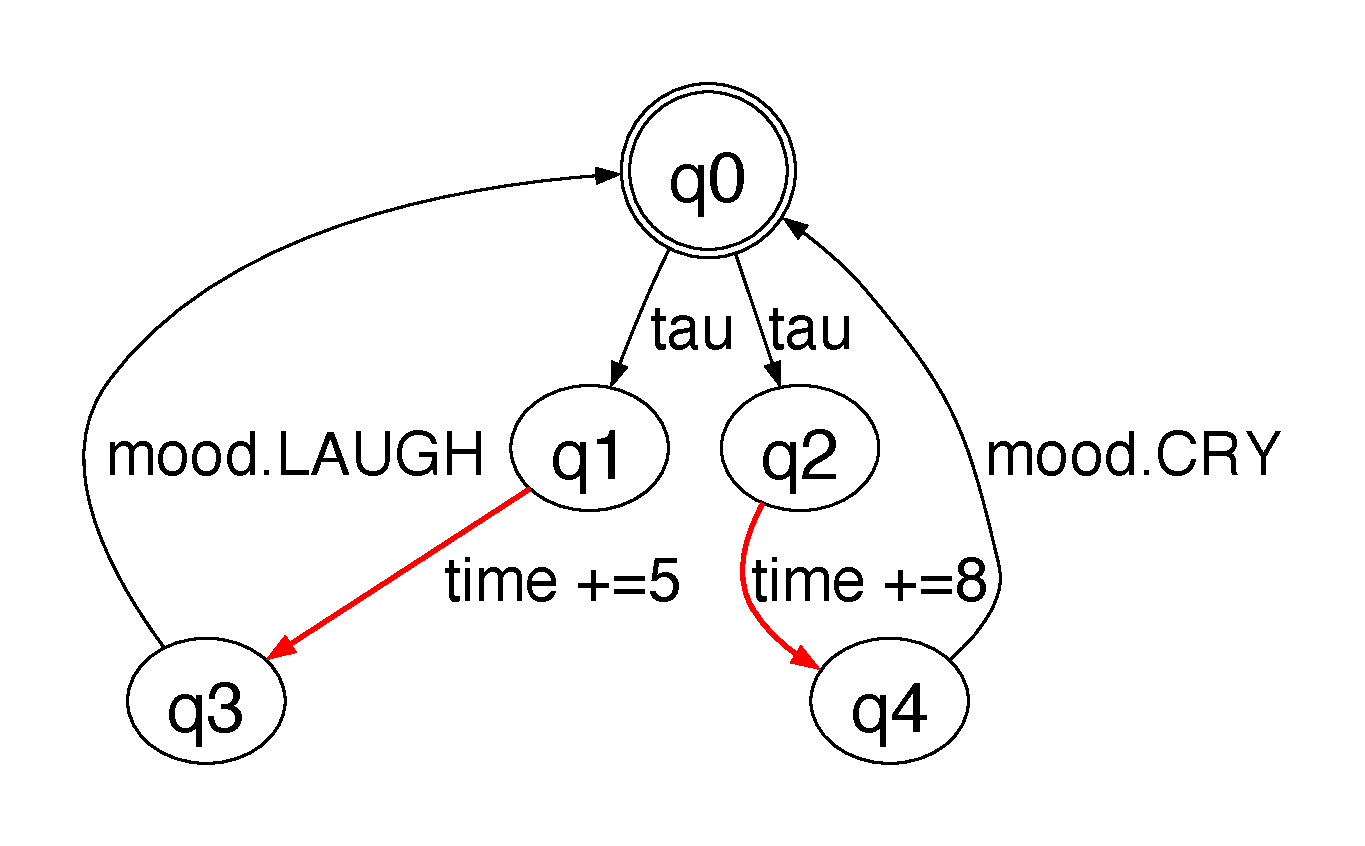
\includegraphics[width=9.9cm]{assets/figures/mood-quotient.pdf}\par
\vspace{.20cm}
{\fontsize{22}{27}\selectfont\color{PosterGreen}\bfseries
 مدل خارج‌قسمتی وارسی‌شده\par}
{\fontsize{19}{24}\selectfont ۵ حالت، ۶ گذار\par}}

\vspace{.22cm}
{\centering\fontsize{18}{24}\selectfont
یال‌های قرمز و ضخیم گذر زمان‌اند و $\tau$ کنش داخلی پنهان‌شده است. مقدار کاهش به
مجموعهٔ مشاهده وابسته است: هرچه کنش‌های کمتری قابل مشاهده باشند، کاهش بیشتر است.\par}
}
